\documentclass[12pt,oneside,a4paper]{book}


\usepackage{polski}
\usepackage[utf8]{inputenc}
\usepackage{lmodern}
\usepackage{titlesec}
\usepackage{fancyhdr}
\usepackage{float}
\titleformat{\chapter}[display]
{\normalfont\bfseries}{}{0pt}{\Large}

\usepackage{amssymb}

\usepackage{geometry}

\usepackage{xcolor}
\usepackage{listings}
\lstset{basicstyle=\ttfamily,
  showstringspaces=false,
  commentstyle=\color{red},
  keywordstyle=\color{blue}
}


\newgeometry{tmargin=2.5cm, bmargin=2.5cm, headheight=14.5pt, inner=3cm, outer=2.5cm} 

\linespread{1.1}

\titlespacing*{\chapter}{0pt}{-60pt}{20pt}

\usepackage{graphicx}
\graphicspath{ {./images/} }

\usepackage{etoolbox}
\makeatletter
\patchcmd{\scr@startchapter}{\if@openright\cleardoublepage\else\clearpage\fi}{}{}{}
\makeatother


\begin{document}
\thispagestyle{empty}
\begin{center}{\sc \Large
Politechnika Warszawska\\}\par\vspace{0.2cm}\par
{\large
Wydział Elektryczny
}
\end{center}
\vspace{5cm}
\begin{center}
{
Uladzislau Hubar, Oleksandr Kolomiiets,\\Yanina Shchaslyva, Lizaveta Niamera, Jan Konarski
}\par\vspace{1 cm}\par
{\LARGE
,,Hurtownie Danych. Projekt\\Bitcoin Blockchain ETL''
}
\end{center}
\vspace{4cm}
\begin{flushright}
Sprawdzający:\\
mgr inż. Krzysztof Marek
\end{flushright}
\vfill
\begin{center}
Warszawa 2021
\end{center}

\thispagestyle{empty} \setcounter{page}{0}

\tableofcontents

\thispagestyle{empty} \setcounter{page}{1}

\newpage

\chapter{Opis projektu}

\section{Cel projektu}
Celem projektu jest zaimplementowanie procesu ,,Extract, Transform and Load'' (ETL) dla danych z Blockchain'u kryptowaluty Bitcoin. Jako efekt końcowy, będzie przedstawiony system, umożliwiający automatyczne pobieranie danych z Blockchain'u, klasteryzację danych oraz zamieszczenie przetransformowanych danych w bazie danych. Przechowywanie przetworzonych danych w bazie umożliwi łatwe pobieranie potrzebnych danych do dalniejszych analiz.
\newline \newline
W celu ułatwienia zadania, skorzystamy z ogólnodostępnego opisu realizacji procesu ETL dla Blockchain'a [1], natomiast bardziej się skupimy na praktycznej realizacji.

\section{Wstęp teoretyczny}
\textbf{Pobieranie (Extract):}
\newline
Dane wejściowe będą pobierane z serwisu \textbf{Blokchain.info}.
\newline \newline
W celu łatwiejszego przetwarzania danych, pobierane będą 150 bloków informacji naraz (informacja o transakcjach za 1 dzień).
\newline \newline
\textbf{Transformacja (Transformation):}
\newline
Proces transformacji danych polega na zastosowaniu algorytmu Klasteryzacji, którego celem będzie zgrupowanie danych o transakcjach dla jednakowych adresów. Algorytm klasteryzacji składa z kilku różnych algorytmów:
\begin{enumerate}
    \item Algorytmu wyszukiwania transakcji
    \item Algorytmu wyszukiwania adresów
    \item Algorytmu aktualizacji
\end{enumerate}

\newpage

\textbf{Algorytm klasteryzacji (Clustering algorithm)}
\newline
\begin{figure}[H]
    \centering
    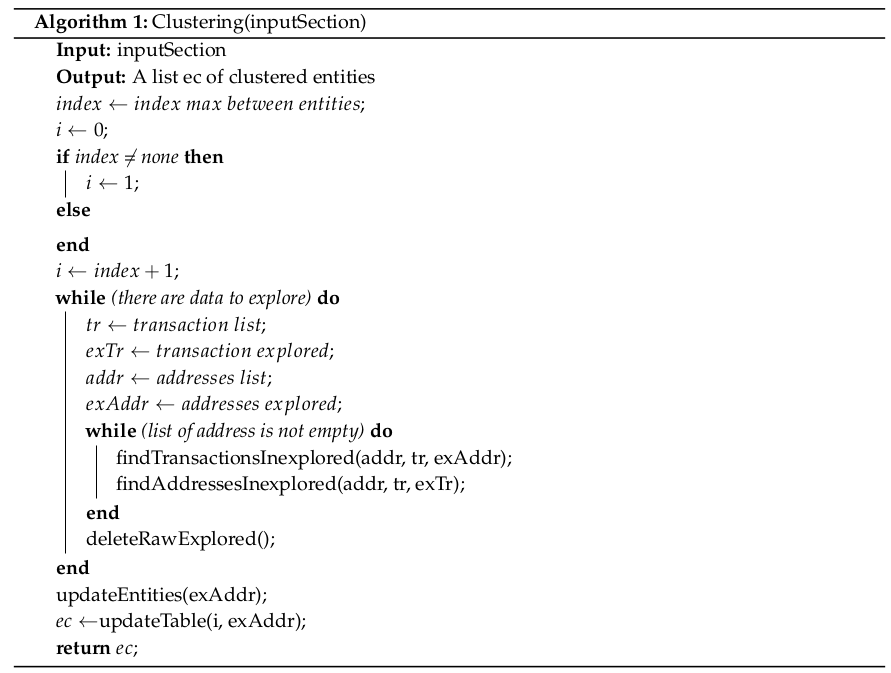
\includegraphics[scale=0.65]{Clustering-alg}
    \caption{Pseudokod algorytmu klasteryzacji [1]}
\end{figure}
\textbf{Algorytm wyszukiwania transakcji (Transaction search algorithm)}
\newline
\begin{figure}[H]
    \centering
    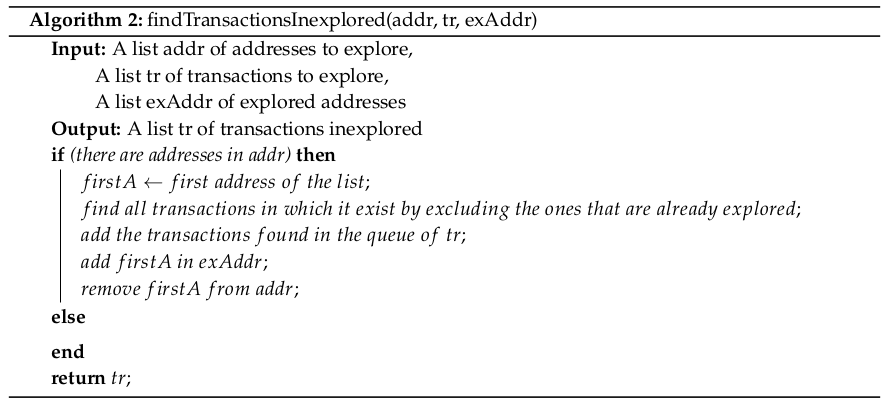
\includegraphics[scale=0.65]{TS-alg}
    \caption{Pseudokod algorytmu wyszukiwania transakcji [1]}
\end{figure}
\textbf{Algorytm wyszukiwania adresów (Adress search algorithm)}
\newline
\begin{figure}[H]
    \centering
    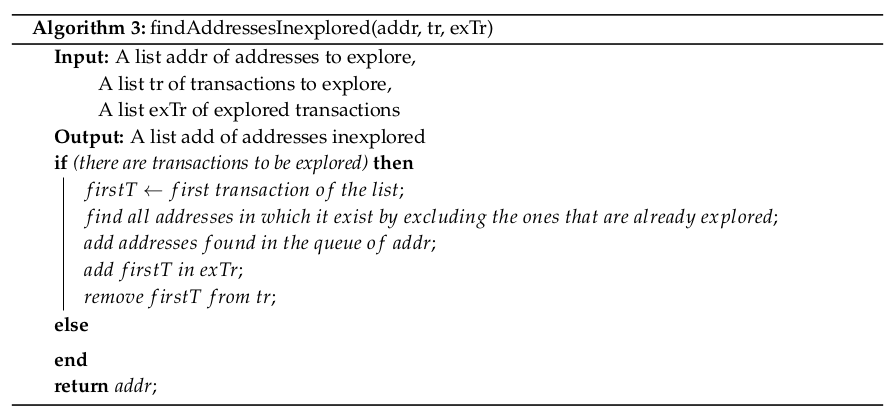
\includegraphics[scale=0.65]{AS-alg}
    \caption{Pseudokod algorytmu wyszukiwania adresów [1]}
\end{figure}
\textbf{Algorytm aktualizacji (Updating Algorithm)}
\newline
\begin{figure}[H]
    \centering
    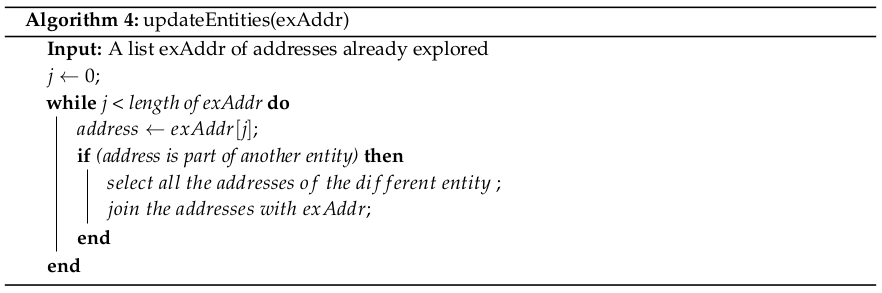
\includegraphics[scale=0.65]{UA-alg}
    \caption{Pseudokod algorytmu aktualizacji [1]}
\end{figure}

\newpage

\textbf{Ładowanie (Load):}
\newline
Ładowanie przetwarzanych danych będzie polegało na zamieszczeniu danych w odpowiednio zaprojektowanej relacyjnej bazie danych.
\newline
Architektura bazy danych:
\begin{figure}[H]
    \centering
    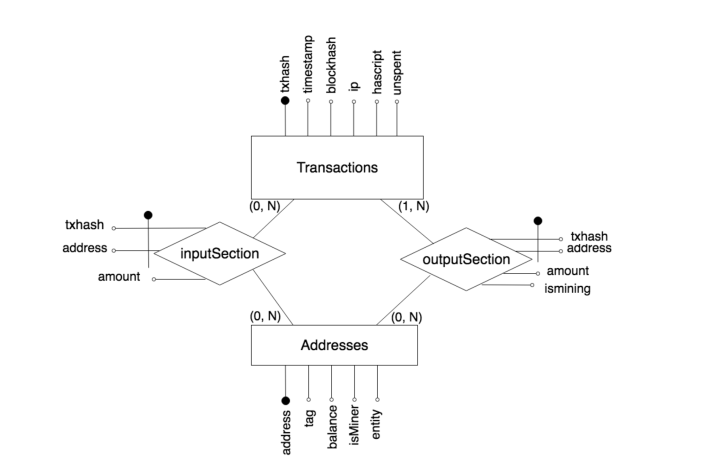
\includegraphics[scale=0.8]{BD-architecture}
    \caption{E-R diagram relacyjnej bazy danych [1]}
\end{figure}
Poniżej jest przedstawiony schemat przebiegu procesu ETL:
\begin{figure}[H]
    \centering
    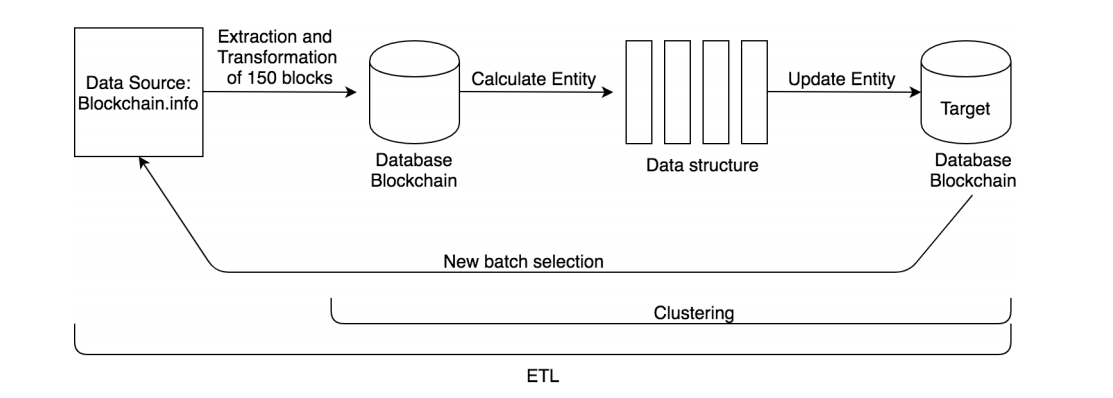
\includegraphics[scale=0.5]{ETL-workflow}
    \caption{Przebieg procesu ETL [1]}
\end{figure}

\newpage

\section{Wykorzystywane narzędzia}
\begin{itemize}
    \item Język programowania: Python
    \item Baza danych: PostgreSQL
    \item HTTP biblioteka: requests
    \item Operacje na haszach: hashlib
    \item Logowanie: logging
    \item Parser parametrów: argparse
\end{itemize}

\chapter{Literatura}
\textit{\textbf{Artykuł}}
\newline
1. Applying the ETL Process to Blockchain Data.
Prospect and Findings
\newline
Roberta Galici, Laura Ordile, Michele Marchesi, Andrea Pinna and Roberto Tonelli


\end{document}
